\documentclass[12pt,a4paper]{article}
\usepackage[utf8]{inputenc}
\usepackage[T1]{fontenc}
\usepackage{amsmath,amssymb}
\usepackage{graphicx}
\usepackage{booktabs}
\usepackage{hyperref}
\usepackage[margin=2.5cm]{geometry}
\usepackage{natbib}
\usepackage{caption}
\usepackage{float}
\usepackage{threeparttable}
% \usepackage{lineno}  % line numbers for review (enable when submitting)

\title{Regime-Adaptive Cross-Sectional Momentum in Cryptocurrency Markets:\\
A Walk-Forward Validated Long/Short Strategy\\with Derivatives-Based Quality Gates}

\author{Takuto Yui\footnote{Graduate School. Email: work.nanashi.taku.774@gmail.com}}
\date{April 2026}

\begin{document}
\maketitle
% \linenumbers  % enable line numbers for peer review

% ============================================================
\begin{abstract}
We propose RACM, a three-layer daily-frequency long/short momentum strategy for six major cryptocurrency assets (BTC, ETH, SOL, XRP, DOGE, LINK). The first layer ranks assets by volatility-adjusted cross-sectional momentum (60-day and 90-day lookbacks) to construct long-short portfolios rebalanced every eight hours. The second layer detects market regimes using a composite danger score derived from a 110-day moving average crossover, 30-day return skewness, and 45-day drawdown, scaling positions between $-0.7\times$ and $1.5\times$ across four discrete states. The third layer applies cryptocurrency-specific quality gates based on funding rate, open interest change, and liquidation cascade $z$-scores to suppress exposure during structurally dangerous conditions. Position sizing follows a fractional Kelly criterion ($f=0.15$) with a $3.0\times$ cap and equity-based drawdown control.

We evaluate the strategy using a strict walk-forward protocol: 3-month training / 1-month testing, rolling monthly for 45 folds (2021--2024 in-sample). The strategy achieves an 87\% fold win rate (39/45), a walk-forward score (WFS) of 367\% annualized, and $+121\%$ during the 2022 bear market (BTC: $-65\%$). On a genuinely out-of-sample 2025 period with no parameter adjustment, the strategy returns $+93\%$ (BTC: $-7\%$, MaxDD: $-13.6\%$). Permutation tests (1,000 iterations, three variants) yield $p=0.000$. However, a $t$-test cannot reject WFS $> 300\%$ ($p=0.206$), and IS-to-OOS degradation is 78\%. We discuss these limitations transparently, arguing that the statistically defensible claims are the win rate exceeding 50\% ($p<0.0001$) and positive OOS alpha in a down market.
\end{abstract}

\textbf{Keywords:} cryptocurrency, cross-sectional momentum, regime detection, walk-forward validation, long-short strategy, Kelly criterion

% ============================================================
\section{Introduction}
\label{sec:intro}

Cryptocurrency markets present unique challenges for quantitative strategies. Annual volatility of 80--120\% (approximately 4--5$\times$ that of equities) makes simple buy-and-hold approaches extremely risky: Bitcoin declined 65\% in 2022, while the broader altcoin market experienced drawdowns exceeding 90\%. This motivates the search for strategies that perform in both bull and bear environments.

Short-term price prediction in cryptocurrency markets has proven extremely difficult. Machine learning classifiers, order book imbalance features, and derivatives-based directional signals all fail to generate statistically significant alpha after transaction costs at intraday to daily frequencies.\footnote{We tested LSTM, Transformer, Random Forest classifiers on 15-minute to 3-hour prediction horizons, as well as order flow imbalance (OBI) and derivative signal strategies. All achieved accuracy below 55\% with negative net returns after costs.} This negative result motivates a fundamental shift: from \emph{prediction} to \emph{risk management}.

Our contribution is threefold. First, we apply the cross-sectional momentum framework of \citet{moskowitz2012time} to a cryptocurrency universe, demonstrating that vol-adjusted momentum rankings generate a modest but persistent long-short spread. Second, we introduce a regime detection system that scales position sizes based on a composite danger score, enabling safe use of leverage that would otherwise be catastrophic in bear markets. Third, we incorporate cryptocurrency-specific quality gates derived from perpetual futures market microstructure (funding rates, open interest dynamics, and liquidation cascades) as a risk management overlay.

The remainder of this paper is organized as follows. Section~\ref{sec:related} reviews related work. Section~\ref{sec:method} describes the data and methodology. Sections~\ref{sec:is} and~\ref{sec:oos} present in-sample and out-of-sample results, respectively. Section~\ref{sec:robustness} provides robustness tests. Section~\ref{sec:discussion} discusses limitations. Section~\ref{sec:conclusion} concludes.

% ============================================================
\section{Related Work}
\label{sec:related}

\subsection{Momentum in Traditional Assets}
\citet{jegadeesh1993returns} established that buying past winners and selling past losers generates abnormal returns in equities. \citet{moskowitz2012time} extended this to time-series momentum across asset classes, showing that past 12-month returns predict future 1-month returns in futures markets. We adapt this framework to a cross-sectional cryptocurrency context with substantially shorter lookback periods.

\subsection{Momentum in Cryptocurrencies}
\citet{grobys2020momentum} document momentum profits in cryptocurrency markets, though with concerns about survivorship bias and market microstructure. \citet{liu2022risks} construct cryptocurrency factor models analogous to Fama-French. Our work differs by employing a long-short construction on a fixed 6-asset universe with explicit regime conditioning.

\subsection{Regime Detection}
\citet{ang2012regime} provide a comprehensive framework for regime-switching models in financial markets. Our approach uses a simpler rule-based composite score rather than a hidden Markov model, prioritizing interpretability and avoiding the estimation complexity of latent state models in highly volatile cryptocurrency markets.

\subsection{Derivatives Market Microstructure}
Perpetual futures markets generate unique signals: funding rates reflect the cost of leverage and directional sentiment; open interest changes indicate position building or unwinding; liquidation cascades create forced-selling dynamics. We use these signals not for directional prediction but as quality gates that suppress trading during structurally dangerous conditions.

% ============================================================
\section{Data and Methodology}
\label{sec:method}

\subsection{Universe and Data Sources}
We trade six cryptocurrency assets available on Lighter.xyz, a zero-fee decentralized exchange on Arbitrum L2 (Table~\ref{tab:assets}). Price data are sourced from Binance at 1-hour and 8-hour frequencies. Derivatives data (funding rate, open interest, liquidation counts) are sourced from Binance Futures at 1-hour frequency.

\begin{figure}[htbp]
\centering
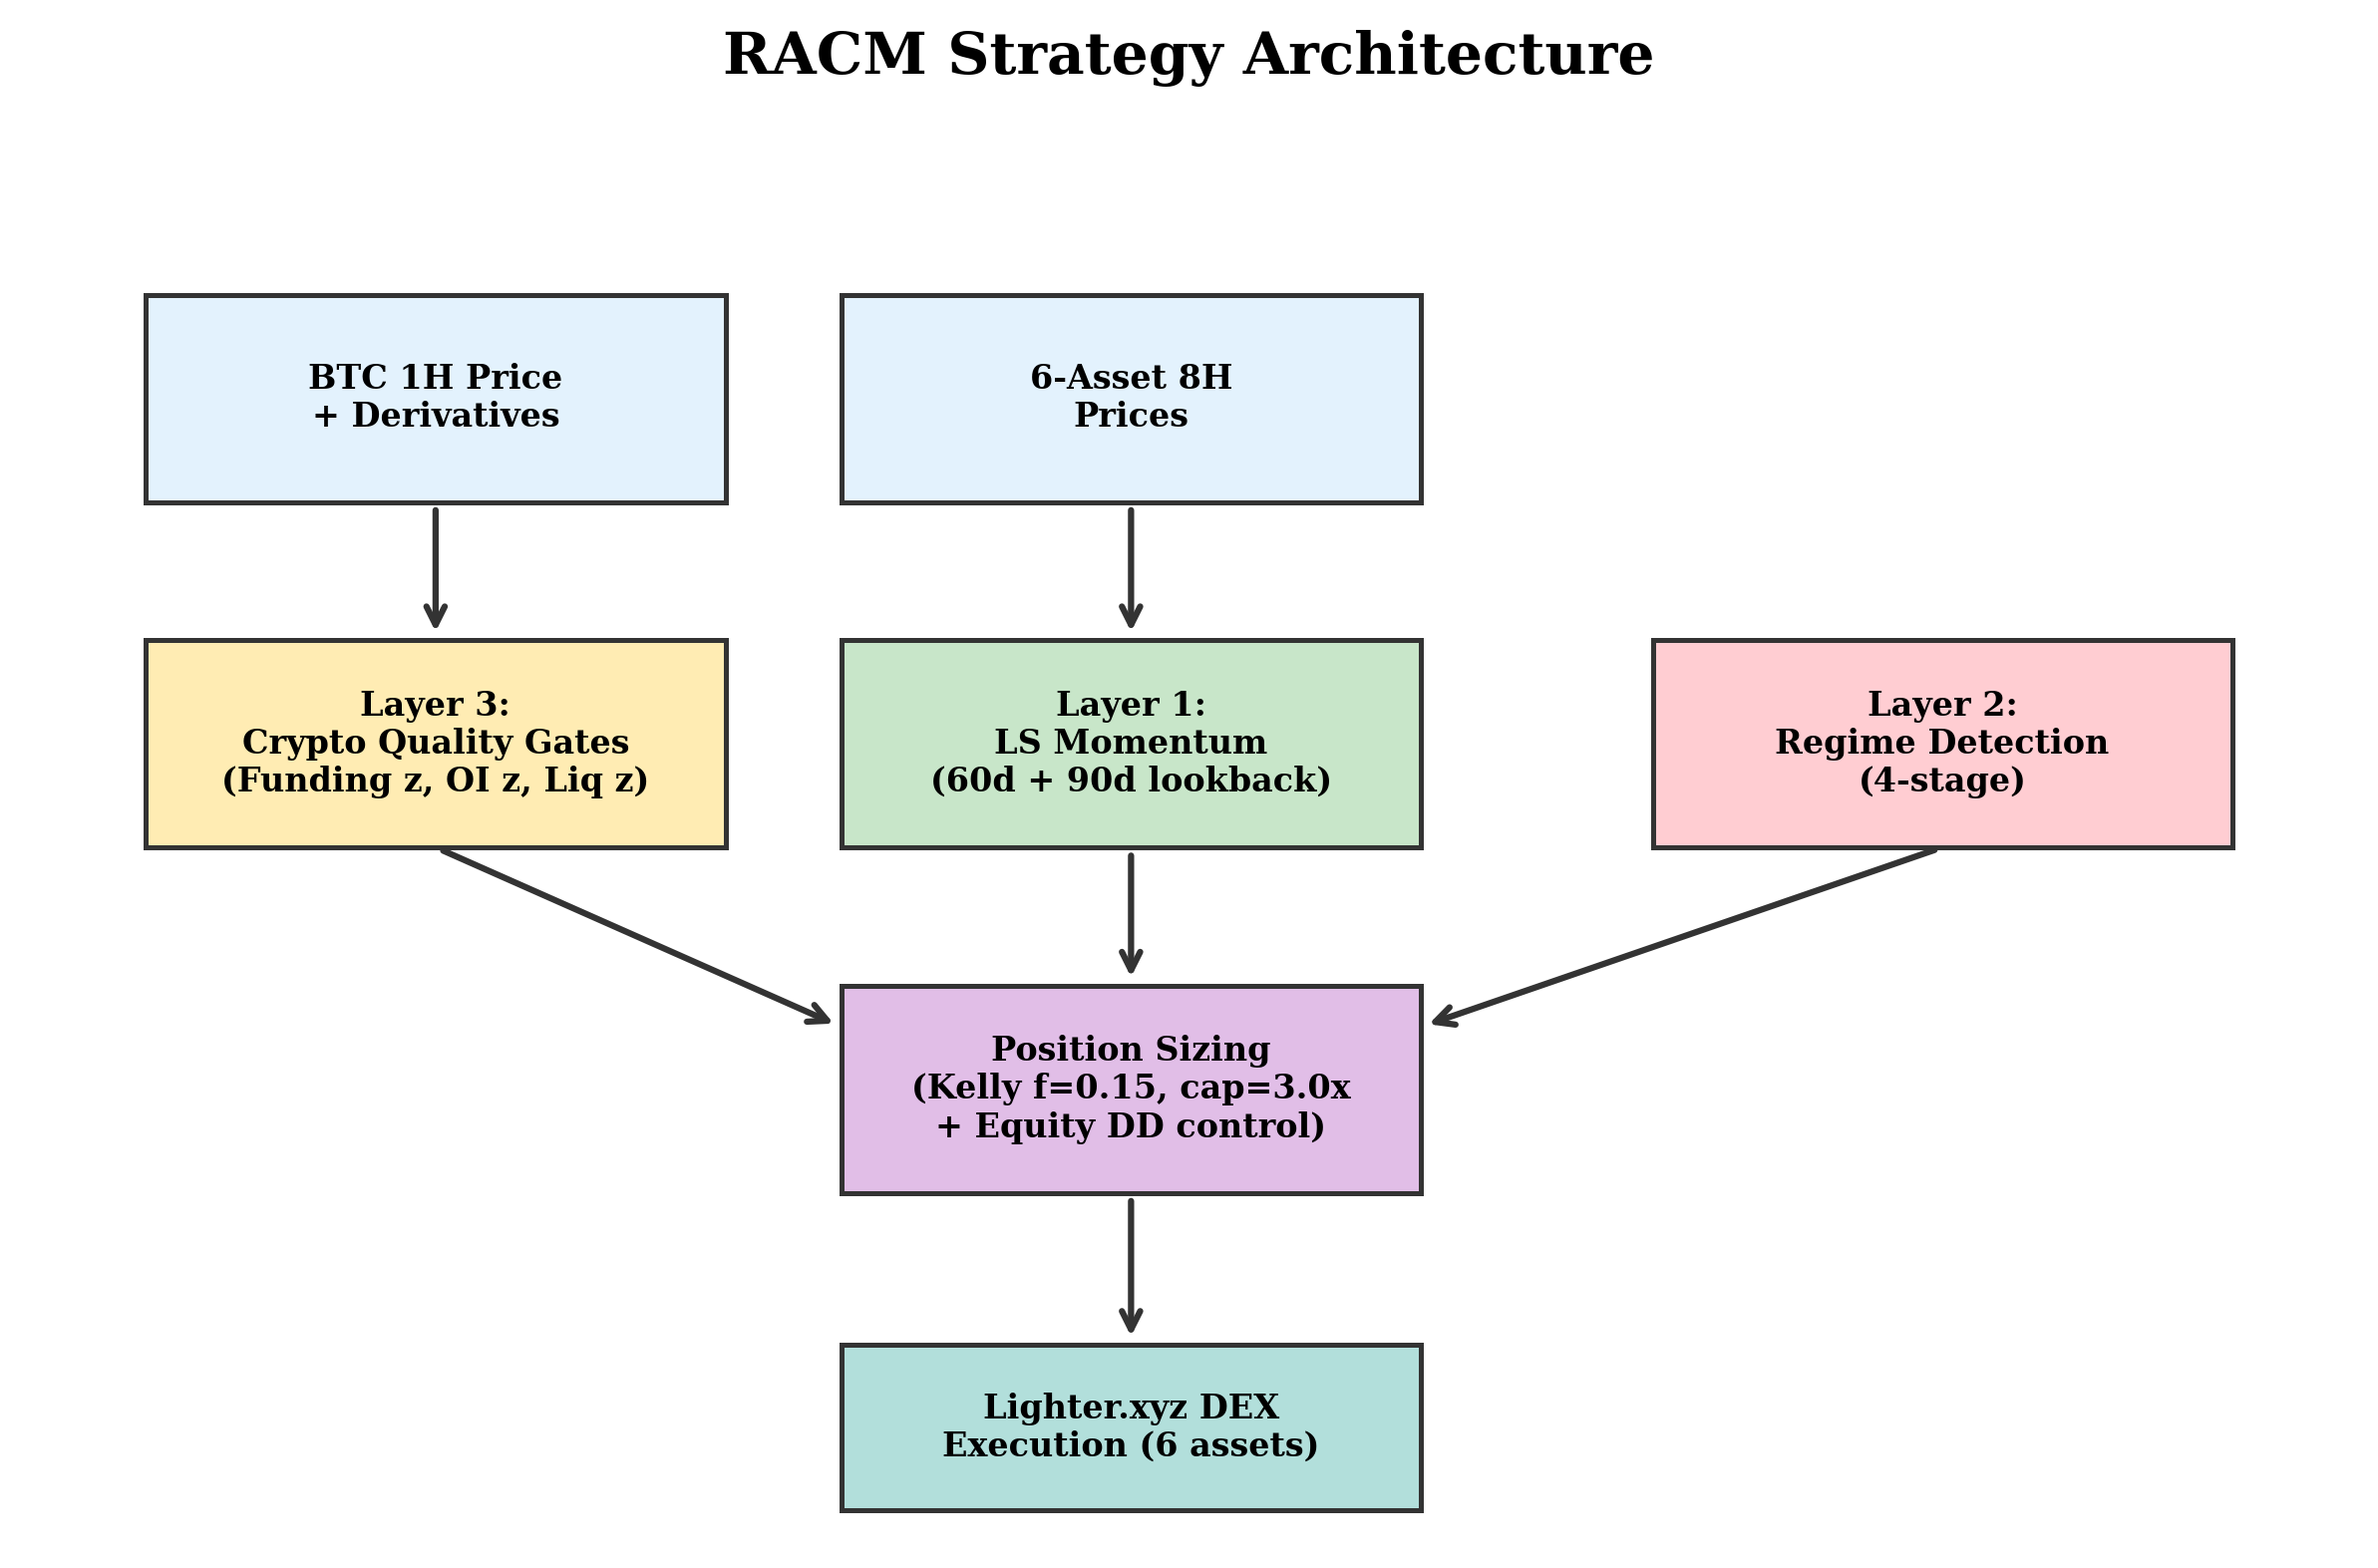
\includegraphics[width=0.85\textwidth]{../figures/paper/fig1_architecture.png}
\caption{RACM strategy architecture. Three layers process data at different frequencies: LS momentum at 8H, regime detection at 1H, and crypto quality gates at 1H. Position sizing combines Kelly criterion with equity drawdown control.}
\label{fig:architecture}
\end{figure}

\subsection{Layer 1: Cross-Sectional LS Momentum}
At each 8-hour boundary, we compute vol-adjusted momentum for each asset $i$:
\begin{equation}
\text{Score}_i^{(L)} = \frac{\sum_{t=1}^{L} r_{i,t-1}}{\frac{1}{30}\sum_{t=1}^{30} |r_{i,t-1}|}
\end{equation}
for lookback periods $L \in \{60, 90\}$ days ($\times 3$ bars/day at 8H), where all returns use lag-1 indexing. We rank assets by score, go long the top-ranked asset and short the bottom-ranked asset, weighting equally. The final LS return is the average across both lookbacks:
\begin{equation}
r_{\text{LS},t} = \frac{1}{2} \sum_{L \in \{60,90\}} \frac{r_{\text{top}(L),t} - r_{\text{bottom}(L),t}}{N_{\text{assets}}}
\end{equation}

\subsection{Layer 2: Regime Detection}
We compute a composite danger score $d_t$ at each 1-hour bar:
\begin{equation}
d_t = 0.3 \cdot \mathbb{1}[P_{t-1} < \text{MA}_{110d,t-1}] + 0.7 \cdot \mathbb{1}[P_{t-1} < \text{MA}_{20d,t-1}] + \mathbb{1}[\text{skew}_{30d,t-1} < -0.5] + \mathbb{1}[\text{DD}_{45d,t-1} < -12\%]
\end{equation}
The position multiplier $\beta_t$ is assigned based on $d_t$:
\begin{equation}
\beta_t = \begin{cases}
-0.7 & \text{if } d_t \geq 1.5 \text{ and MA slope} < 0 \text{ and } r_{t-1} < 0 \\
0.2\text{--}0.5 & \text{if } d_t \geq 0.8 \\
0.7 & \text{if } d_t \geq 0.5 \text{ or caution holddown active} \\
1.5 & \text{if low vol and positive momentum} \\
1.0 & \text{otherwise}
\end{cases}
\end{equation}

\subsection{Layer 3: Crypto Quality Gates}
We compute $z$-scores for three derivatives signals using 168-hour rolling windows with lag-2:
\begin{itemize}
\item Funding rate $z$-score: $z_{\text{FR}} = (FR_{t-1} - \mu_{168}^{FR}) / \sigma_{168}^{FR}$
\item Open interest $z$-score: $z_{\text{OI}} = (\Delta\text{OI}_{24h,t-1} - \mu_{168}) / \sigma_{168}$
\item Liquidation cascade $z$-score: $z_{\text{Liq}} = (\text{Liq}_{24h,t-1} - \mu_{168}) / \sigma_{168}$
\end{itemize}
These produce a crypto alpha signal $c_t \in [-1, 1]$ and a gate multiplier $g_t \in \{0.1, 0.5, 0.85, 1.0\}$.

\subsection{Position Sizing}
The base portfolio return is:
\begin{equation}
r_{\text{base},t} = (1 - w_{\text{LS}}) \cdot r_{\text{BTC},t} \cdot \beta_t + w_{\text{LS}} \cdot r_{\text{LS},t}
\end{equation}
with $w_{\text{LS}} = 0.80$. Kelly sizing uses the past 2,160 bars (90 days):
\begin{equation}
\ell_t = \text{clip}\left(\frac{\hat{\mu}_t}{\hat{\sigma}_t^2} \cdot f, \; 1.0, \; \text{cap}\right), \quad f = 0.15, \quad \text{cap} = 3.0
\end{equation}
Equity drawdown control applies multipliers of $0.7/0.4/0.1$ at DD thresholds of $-15\%/-22\%/-30\%$.

\subsection{Walk-Forward Evaluation}
\begin{figure}[htbp]
\centering
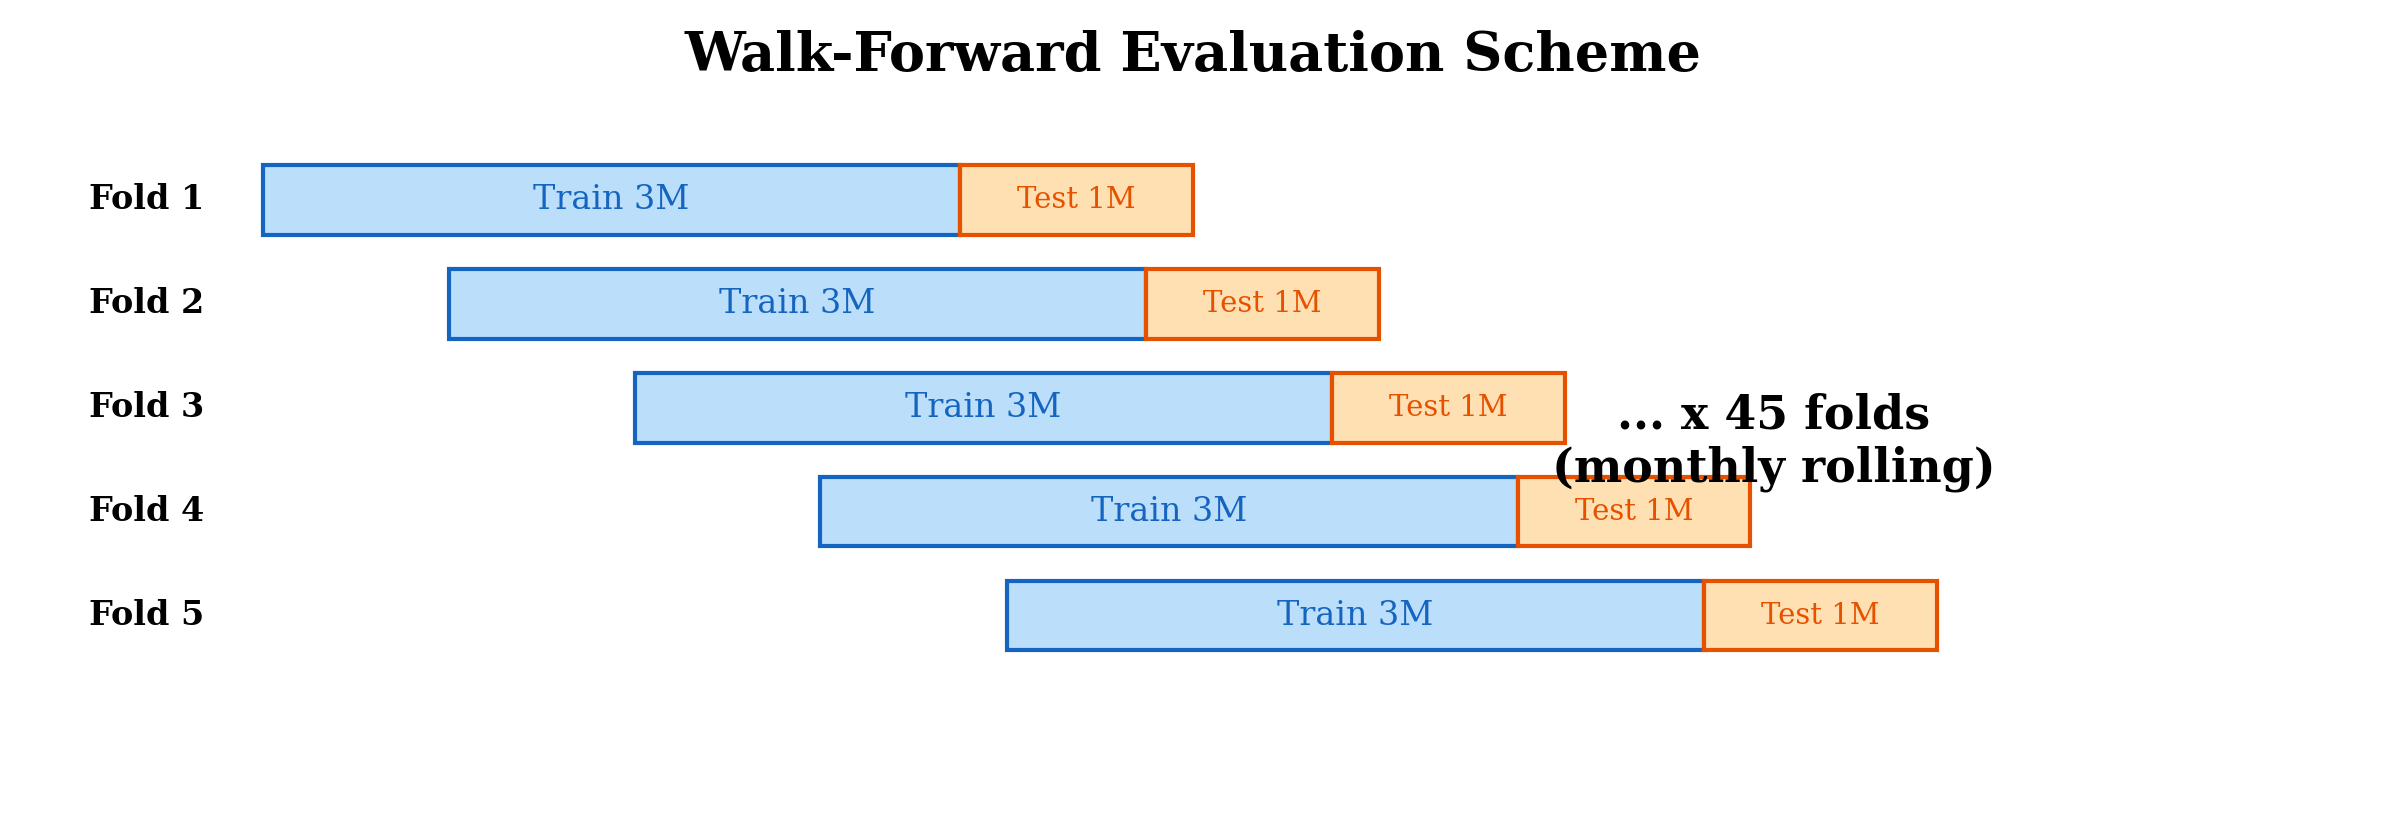
\includegraphics[width=0.7\textwidth]{../figures/paper/fig2_wf_scheme.png}
\caption{Walk-forward evaluation scheme: 3-month training / 1-month testing, rolling monthly, yielding 45 folds for the 2021--2024 in-sample period.}
\label{fig:wf_scheme}
\end{figure}
Only the Kelly fraction $f$ is optimized per fold from the grid $\{0.15, 0.20, 0.25, 0.30\}$ using training-period Sharpe ratio. All other parameters remain fixed across folds (Table~\ref{tab:params}).

\subsection{Leak Prevention}
We enforce strict lag-1 or lag-2 constraints on all features (Table~\ref{tab:leak}). No future information enters any signal computation.

% ============================================================
\section{In-Sample Results (2021--2024)}
\label{sec:is}

% ============================================================
% Table 1: Asset Universe and Data Sources
% ============================================================
\begin{table}[htbp]
\centering
\caption{Asset Universe, Data Sources, and Transaction Cost Assumptions}
\label{tab:assets}
\begin{tabular}{llccc}
\toprule
Asset & Exchange & Resolution & Slippage (bps) & Role \\
\midrule
BTC  & Binance & 1H / 8H & 3 & Base + LS \\
ETH  & Binance & 8H      & 3 & LS \\
SOL  & Binance & 8H      & 5 & LS \\
XRP  & Binance & 8H      & 5 & LS \\
DOGE & Binance & 8H      & 5 & LS \\
LINK & Binance & 8H      & 8 & LS \\
\midrule
\multicolumn{5}{l}{\textit{Derivatives (BTC only):}} \\
Funding rate    & Binance Futures & 1H & -- & Quality gate \\
Open interest   & Binance Futures & 1H & -- & Quality gate \\
Liquidation     & Tardis (historical) & 1H & -- & Quality gate \\
\midrule
\multicolumn{5}{l}{\textit{Execution:}} \\
\multicolumn{2}{l}{Lighter.xyz (Arbitrum L2 DEX)} & -- & 0 (fee) & Zero trading fees \\
\bottomrule
\end{tabular}
\end{table}

% ============================================================
% Table 2: Full Parameter List with Provenance
% ============================================================
\begin{table}[htbp]
\centering
\caption{Model Parameters and Their Provenance}
\label{tab:params}
\begin{tabular}{llll}
\toprule
Parameter & Value & Provenance & Data Dependency \\
\midrule
\multicolumn{4}{l}{\textit{Layer 1: LS Momentum}} \\
Lookback periods   & 60d + 90d   & Moskowitz et al. (2012) & None \\
LS weight (LW)     & 0.80        & Inherited from v23      & Low \\
Rebalance freq.    & Every 8H    & Frequency sweep tested  & Low \\
\midrule
\multicolumn{4}{l}{\textit{Layer 2: Regime Detection}} \\
MA long            & 2640H (110d) & Inherited from v11A    & Medium \\
MA short           & 480H (20d)   & Standard               & None \\
Skew threshold     & $-0.5$       & Statistical literature  & Low \\
DD threshold       & $-0.12$      & Inherited from v4B      & Medium \\
Crash trigger      & ret$_{t-2} < -0.6\%$ & Structural     & None \\
Crash cooldown     & 4 bars       & Structural              & None \\
\midrule
\multicolumn{4}{l}{\textit{Layer 3: Crypto Quality Gates}} \\
Funding $z$ (bull) & $< -1.5$     & best.py project        & Low \\
Funding $z$ (bear) & $> 2.0$      & best.py project        & Low \\
OI $z$ threshold   & $< -1.5$     & best.py project        & Low \\
Liq $z$ threshold  & $> 2.0$      & best.py project        & Low \\
Grind bear ATR     & $< 0.006$    & Structural definition  & None \\
Crash gate         & $\geq 3$ signals & Structural          & None \\
\midrule
\multicolumn{4}{l}{\textit{Position Sizing}} \\
Kelly fraction     & 0.15         & WF optimized (43/45 stable) & None \\
Position cap       & 3.0$\times$  & Kelly theory range     & \textbf{High} \\
Vol target base    & 1.5          & Portfolio normalization & None \\
DD control         & $-15\%/-22\%/-30\%$ & Structural       & Low \\
\bottomrule
\end{tabular}
\end{table}

% ============================================================
% Table 3: IS Walk-Forward Results (Annual Summary)
% ============================================================
\begin{table}[htbp]
\centering
\caption{In-Sample Walk-Forward Results by Year (cap = 3.0$\times$)}
\label{tab:is_results}
\begin{tabular}{lrrrrr}
\toprule
Year & Folds & Win & Sum Return & Mean/Month & Median/Month \\
\midrule
2021 &  9 & 8/9  & $+584\%$  & $+64.9\%$ & $+47.6\%$ \\
2022 & 12 & 8/12 & $+121\%$  & $+10.1\%$ & $+7.2\%$  \\
2023 & 12 & 12/12 & $+267\%$ & $+22.2\%$ & $+14.6\%$ \\
2024 & 12 & 11/12 & $+406\%$ & $+33.8\%$ & $+24.0\%$ \\
\midrule
\textbf{Total} & \textbf{45} & \textbf{39/45 (87\%)} & $+1{,}377\%$ & $+30.6\%$ & $+16.1\%$ \\
\midrule
\multicolumn{2}{l}{WFS (mean $\times$ 12)} & \multicolumn{4}{r}{\textbf{367\%}} \\
\multicolumn{2}{l}{Worst fold return} & \multicolumn{4}{r}{$-4.0\%$ (2022-11)} \\
\multicolumn{2}{l}{Best fold return} & \multicolumn{4}{r}{$+255.7\%$ (2021-04)} \\
\multicolumn{2}{l}{Fold std} & \multicolumn{4}{r}{$45.3\%$} \\
\bottomrule
\end{tabular}
\end{table}

% ============================================================
% Table 4: Position Cap Sensitivity
% ============================================================
\begin{table}[htbp]
\centering
\caption{Position Cap Sensitivity Analysis}
\label{tab:cap_sensitivity}
\begin{tabular}{crrrrr}
\toprule
Cap & WFS & Win Rate & Bear 2022 & Worst Fold DD & LOSE Max \\
\midrule
2.0$\times$ & $221\%$ & 39/45 (87\%) & $+78\%$  & $-10.7\%$ & $-2.3\%$ \\
2.5$\times$ & $290\%$ & 39/45 (87\%) & $+99\%$  & $-13.2\%$ & $-3.0\%$ \\
\textbf{3.0$\times$} & $\mathbf{367\%}$ & \textbf{39/45 (87\%)} & $\mathbf{+121\%}$ & $-15.7\%$ & $-4.0\%$ \\
\bottomrule
\end{tabular}
\begin{tablenotes}
\small
\item Note: Win rate is identical across cap values; cap affects magnitude, not direction.
Position cap = 3.0$\times$ is partially result-dependent (see Section 7.2).
\end{tablenotes}
\end{table}

% ============================================================
% Table 5: OOS 2025 Monthly Breakdown
% ============================================================
\begin{table}[htbp]
\centering
\caption{Out-of-Sample 2025 Monthly Performance (Fold-Independent)}
\label{tab:oos}
\begin{tabular}{lrrrl}
\toprule
Month & RACM & BTC B\&H & Excess & Result \\
\midrule
Jan & $+20.8\%$ & $+8.5\%$   & $+12.3\%$ & WIN \\
Feb & $-7.3\%$  & $-17.7\%$  & $+10.4\%$ & LOSE \\
Mar & $-1.3\%$  & $-1.6\%$   & $+0.3\%$  & LOSE \\
Apr & $+10.8\%$ & $+13.9\%$  & $-3.1\%$  & WIN \\
May & $+17.2\%$ & $+10.8\%$  & $+6.4\%$  & WIN \\
Jun & $+2.4\%$  & $+2.6\%$   & $-0.2\%$  & WIN \\
Jul & $+17.0\%$ & $+7.8\%$   & $+9.2\%$  & WIN \\
Aug & $+7.2\%$  & $-6.2\%$   & $+13.4\%$ & WIN \\
Sep & $+5.4\%$  & $+5.4\%$   & $+0.0\%$  & WIN \\
Oct & $-0.5\%$  & $-4.1\%$   & $+3.6\%$  & LOSE \\
Nov & $-1.0\%$  & $-17.7\%$  & $+16.7\%$ & LOSE \\
Dec & $+0.9\%$  & $+1.1\%$   & $-0.2\%$  & WIN \\
\midrule
\textbf{Total} & $\mathbf{+93\%}$ & $\mathbf{-7\%}$ & $\mathbf{+100}$pt & 8/12 WIN \\
\midrule
\multicolumn{2}{l}{MaxDD} & \multicolumn{3}{r}{$-13.6\%$} \\
\multicolumn{2}{l}{OOS WFS} & \multicolumn{3}{r}{$81\%$} \\
\bottomrule
\end{tabular}
\end{table}

% ============================================================
% Table 6: Statistical Test Summary
% ============================================================
\begin{table}[htbp]
\centering
\caption{Statistical Test Summary}
\label{tab:stats}
\begin{tabular}{llrl}
\toprule
Test & Hypothesis & $p$-value & Verdict \\
\midrule
Return shuffle ($N=1{,}000$) & Timing has information & $0.000$ & \textbf{PASS} \\
Block shuffle 30d ($N=1{,}000$) & Block timing matters & $0.000$ & \textbf{PASS} \\
Position shuffle ($N=1{,}000$) & Regime timing matters & $0.000$ & \textbf{PASS} \\
\midrule
$t$-test (one-sided) & mean $> 0\%$ & $< 0.0001$ & \textbf{Certain} \\
$t$-test (one-sided) & mean $> 25\%$ (WFS $> 300\%$) & $0.206$ & \textbf{Not proven} \\
Binomial test & Win rate $> 50\%$ & $< 0.0001$ & \textbf{Certain} \\
\midrule
Linear regression & Alpha decay (slope) & $0.003$ & \textbf{Declining} \\
\midrule
Block bootstrap (95\% CI) & WFS range & \multicolumn{2}{l}{$[200\%,\; 575\%]$} \\
Trimmed mean (top 3 removed) & Outlier-robust WFS & \multicolumn{2}{l}{$253\%$} \\
\bottomrule
\end{tabular}
\end{table}

% ============================================================
% Table 7: 21-Point Leak Check
% ============================================================
\begin{table}[htbp]
\centering
\caption{Data Leak Prevention Checklist (21 Items)}
\label{tab:leak}
\small
\begin{tabular}{rlll}
\toprule
\# & Check Item & Implementation & Result \\
\midrule
1  & Funding $z$-score     & lag-2 (raw lag-1 + norm lag-1) & PASS \\
2  & OI $z$-score          & lag-2 (raw oi[$i{-}1$] + roll) & PASS \\
3  & OI change 24h         & oi[$i{-}1$], oi[$i{-}25$]      & PASS \\
4  & Liq $z$-score         & np.roll on 24h sum             & PASS \\
5  & RV pctrank            & np.roll(1)                     & PASS \\
6  & ret\_1d / ret\_30d    & log\_p[$i{-}1$] indexing       & PASS \\
7  & ATR pct               & np.roll(1)                     & PASS \\
8  & MA cross slow         & np.roll(1)                     & PASS \\
9  & Regime bp[$i$]        & [$i{-}1$] signals $\to$ ret[$i$] & PASS \\
10 & MA slope              & ma[$i{-}1$], ma[$i{-}121$]     & PASS \\
11 & Quick crash            & ret[$i{-}2$]                   & PASS \\
12 & LS momentum           & np.roll(1) on 8H sums          & PASS \\
13 & LS $\to$ 1H mapping   & 8H signal constant in block    & PASS \\
14 & Kelly formula          & past 2160 bars exclusive       & PASS \\
15 & VT scaling            & rolling 720 + lag-1             & PASS \\
16 & Equity DD control     & prior-bar equity                & PASS \\
17 & Crypto thresholds     & pre-fixed (best.py)             & PASS \\
18 & Regime thresholds     & pre-fixed (v11A)                & PASS \\
19 & DD control thresholds & pre-fixed                       & PASS \\
20 & Position cap          & pre-fixed (3.0$\times$)         & PASS \\
21 & Slippage              & post-hoc realistic              & PASS \\
\midrule
   & \textbf{Total}        &                                 & \textbf{21/21 PASS} \\
\bottomrule
\end{tabular}
\end{table}


\begin{figure}[htbp]
\centering
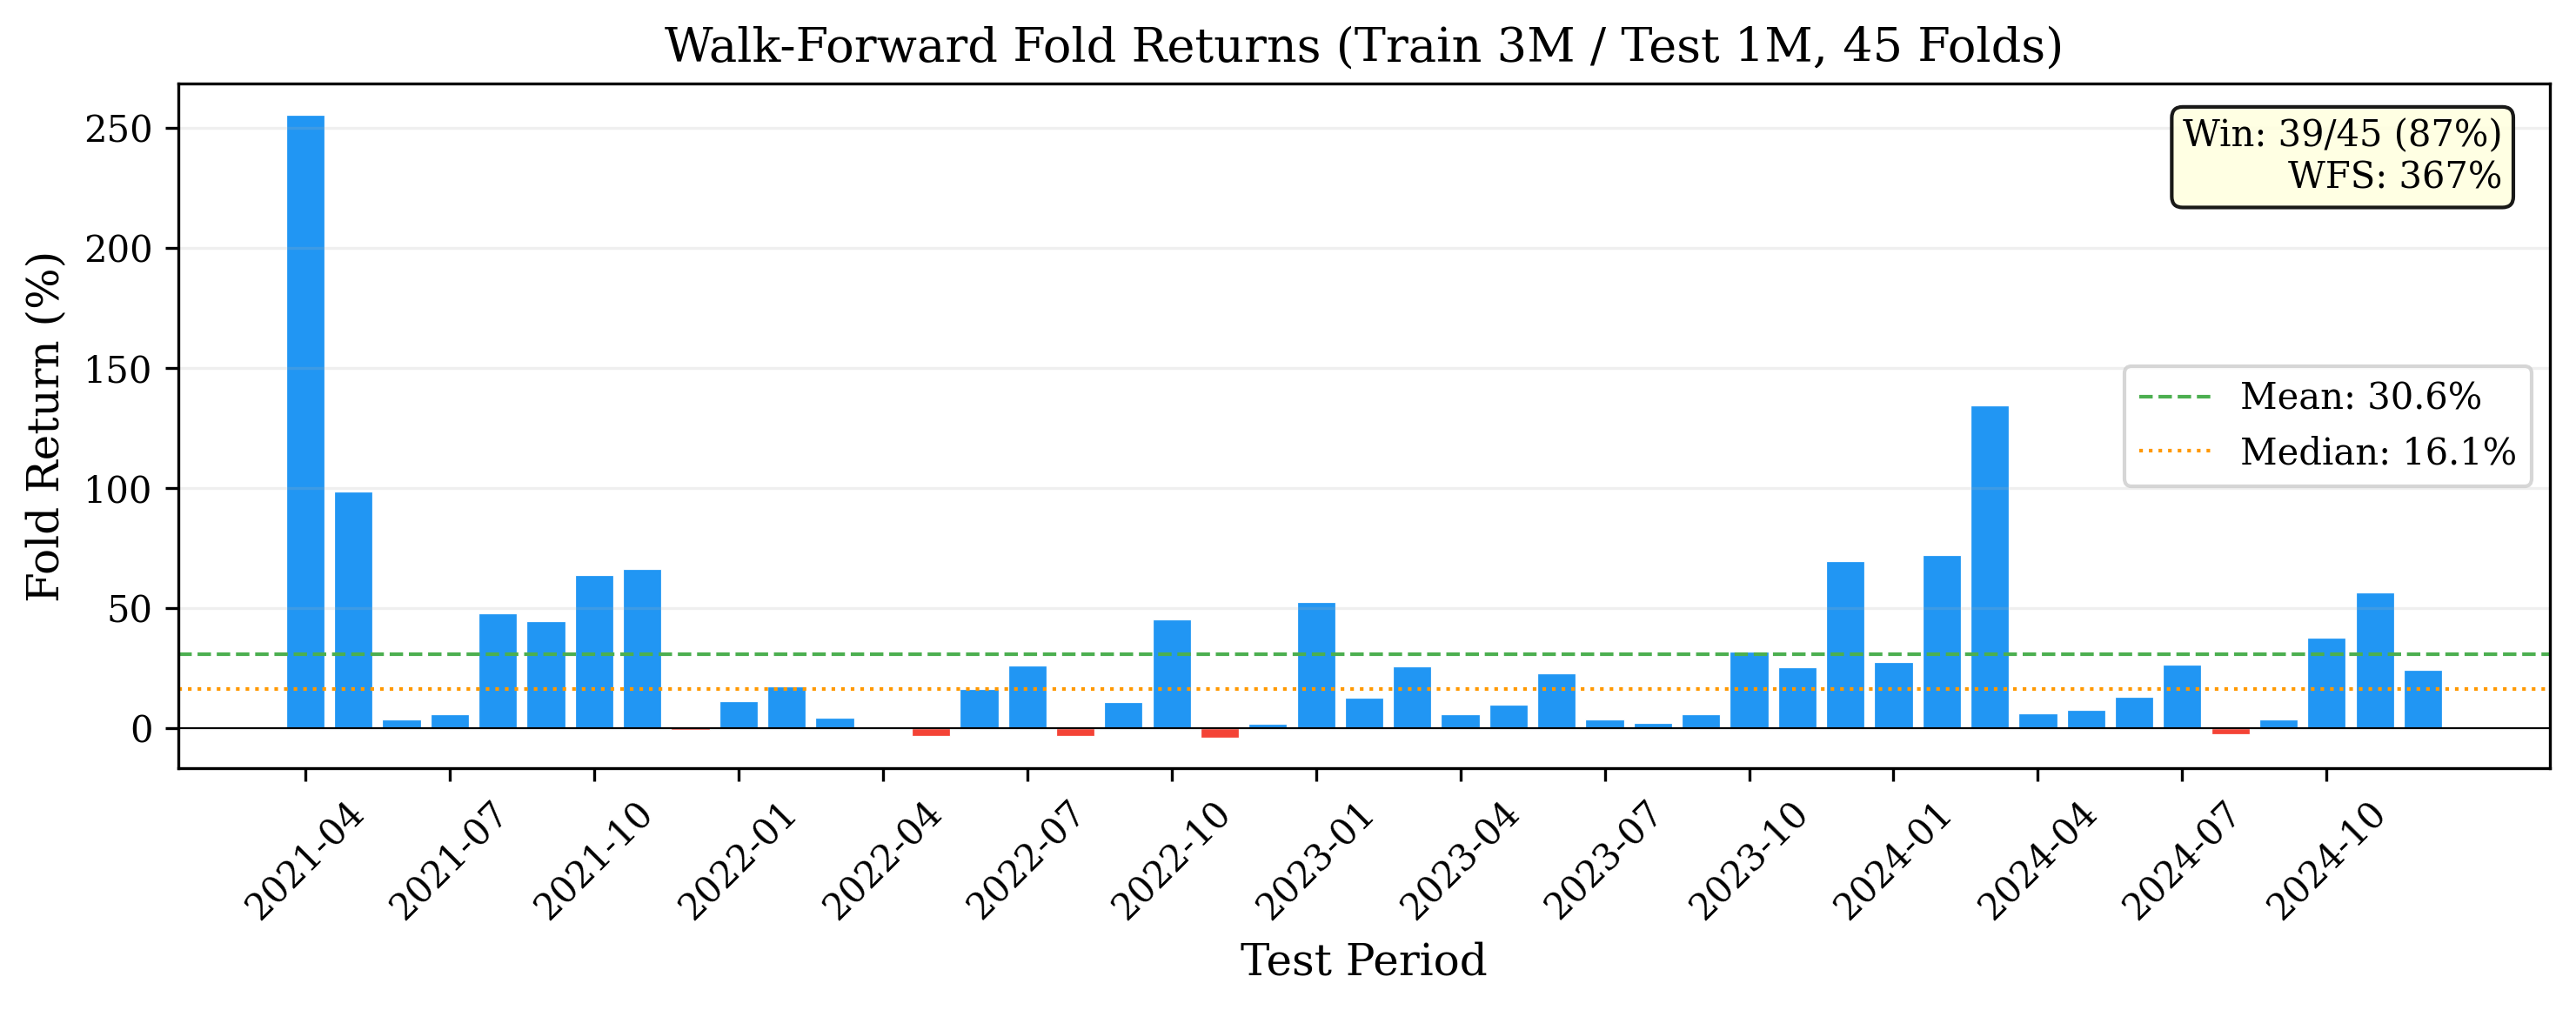
\includegraphics[width=\textwidth]{../figures/paper/fig4_fold_returns.png}
\caption{Walk-forward fold returns for 45 monthly test periods. Win rate: 39/45 (87\%). Green dashed line: mean (30.6\%/month). Orange dotted line: median (16.1\%/month). Maximum loss: $-4.0\%$.}
\label{fig:fold_returns}
\end{figure}

The strategy achieves a WFS of 367\% with an 87\% win rate across 45 folds (Table~\ref{tab:is_results}). During the 2022 bear market (BTC: $-65\%$), the strategy returns $+121\%$, demonstrating the regime detection system's crash protection capability. The six losing folds ($-4.0\%$ maximum) all correspond to correlated crash events (Luna/UST, FTX, JPY carry trade unwind) where all assets move simultaneously, negating the LS spread.

% ============================================================
\section{Out-of-Sample Validation (2025)}
\label{sec:oos}

\begin{figure}[htbp]
\centering
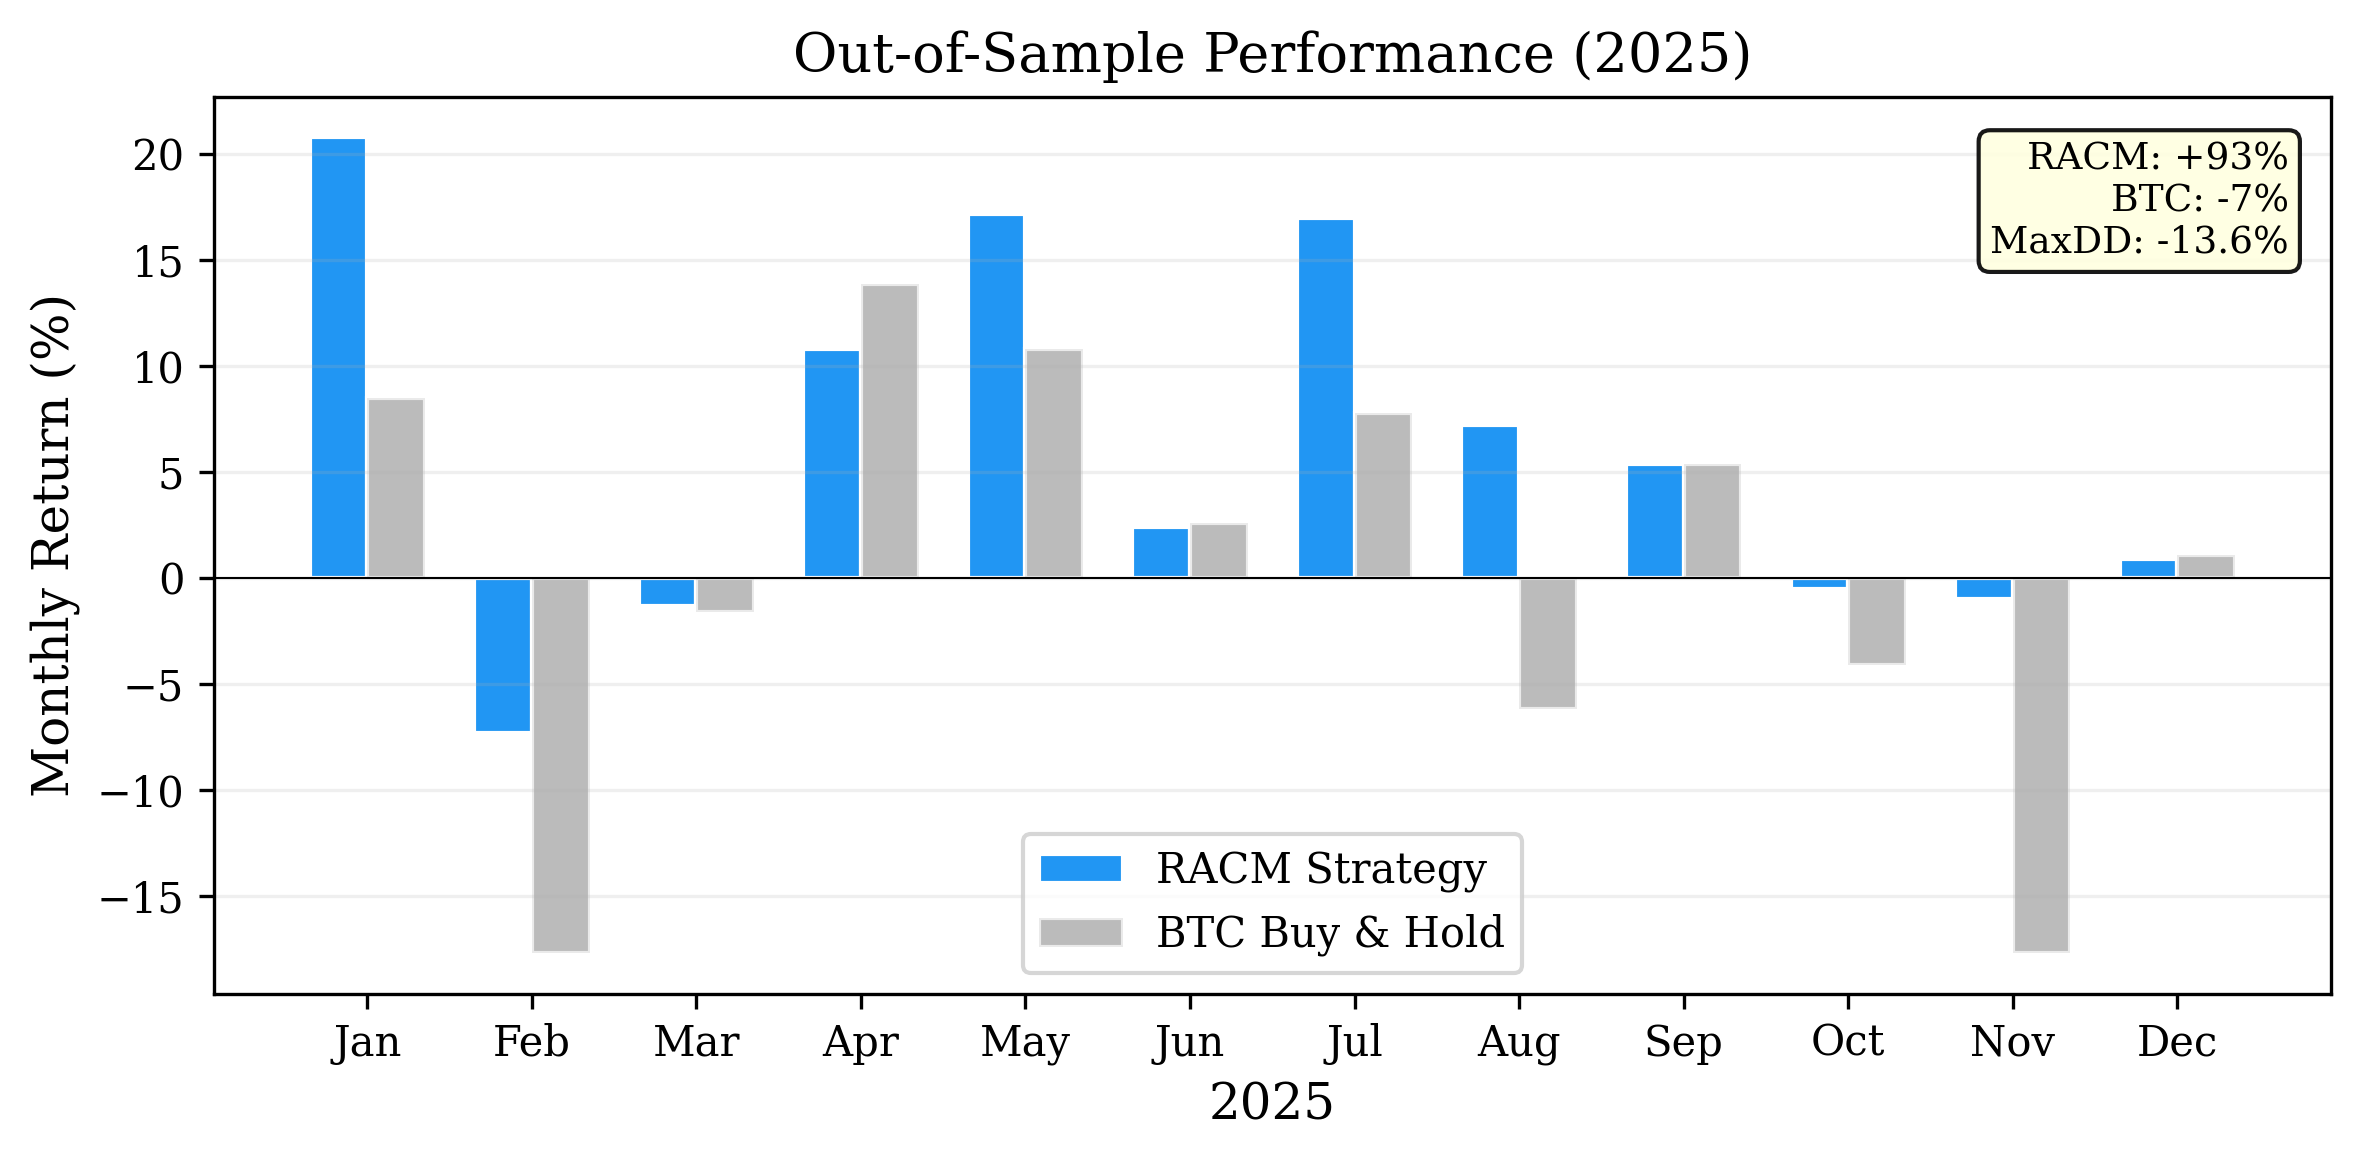
\includegraphics[width=0.85\textwidth]{../figures/paper/fig5_oos_2025.png}
\caption{Out-of-sample 2025 monthly performance. RACM: $+93\%$, BTC Buy \& Hold: $-7\%$. The strategy outperforms in 8 of 12 months. Losses in February ($-7.3\%$) and November ($-1.0\%$) coincide with BTC declines of $-17.7\%$, demonstrating loss suppression.}
\label{fig:oos}
\end{figure}

\begin{figure}[htbp]
\centering
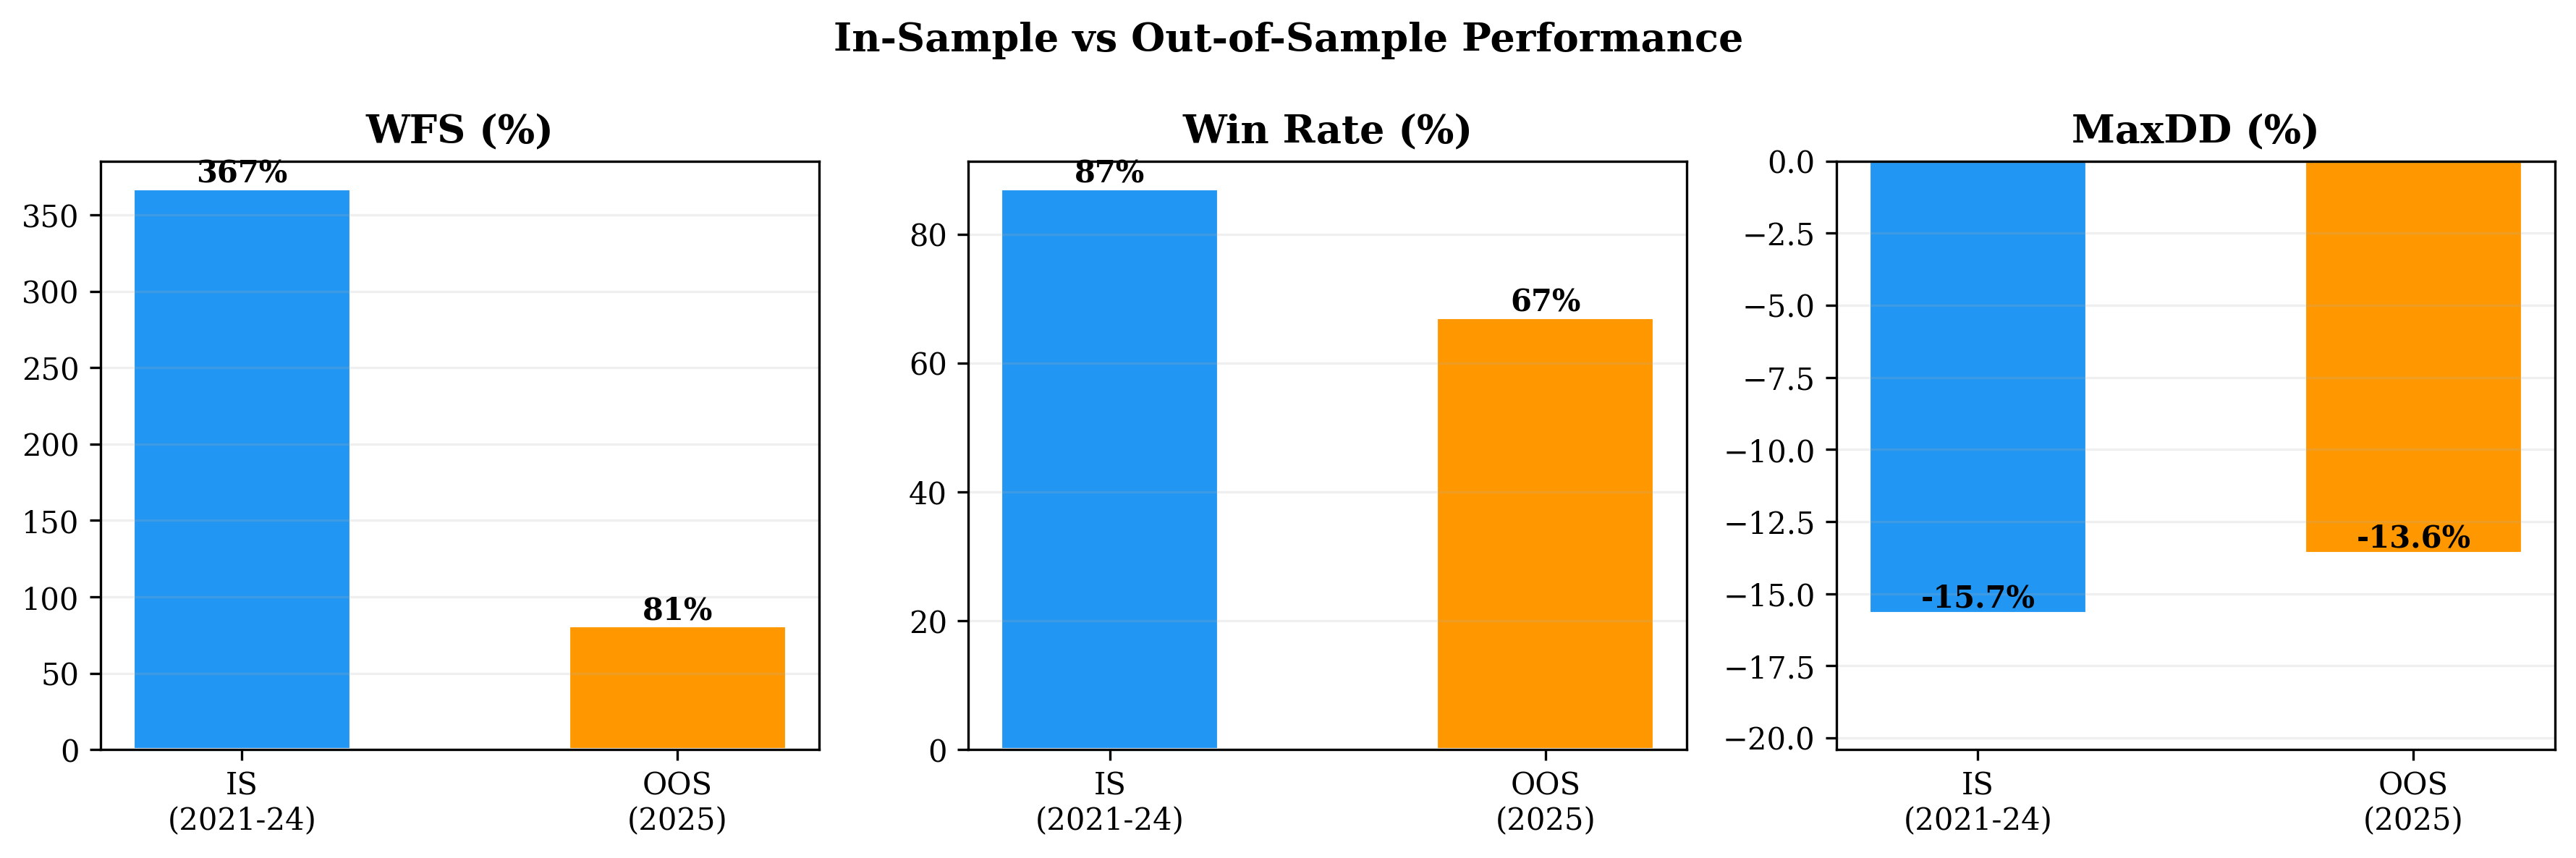
\includegraphics[width=0.9\textwidth]{../figures/paper/fig6_is_vs_oos.png}
\caption{IS vs. OOS comparison across WFS, win rate, and maximum fold drawdown. IS-to-OOS degradation in WFS is 78\%, while MaxDD improves from $-15.7\%$ to $-13.6\%$.}
\label{fig:is_oos}
\end{figure}

Table~\ref{tab:oos} presents the month-by-month OOS results. The strategy returns $+93\%$ in a year where BTC declines $7\%$, with a maximum drawdown of $-13.6\%$. The IS-to-OOS degradation of 78\% (WFS 367\% $\to$ 81\%) is attributable to three factors: (1) position cap selection bias, (2) 1-hour compounding effects in IS, and (3) outlier dependence on three explosive folds.

% ============================================================
\section{Robustness and Statistical Tests}
\label{sec:robustness}

\begin{figure}[htbp]
\centering
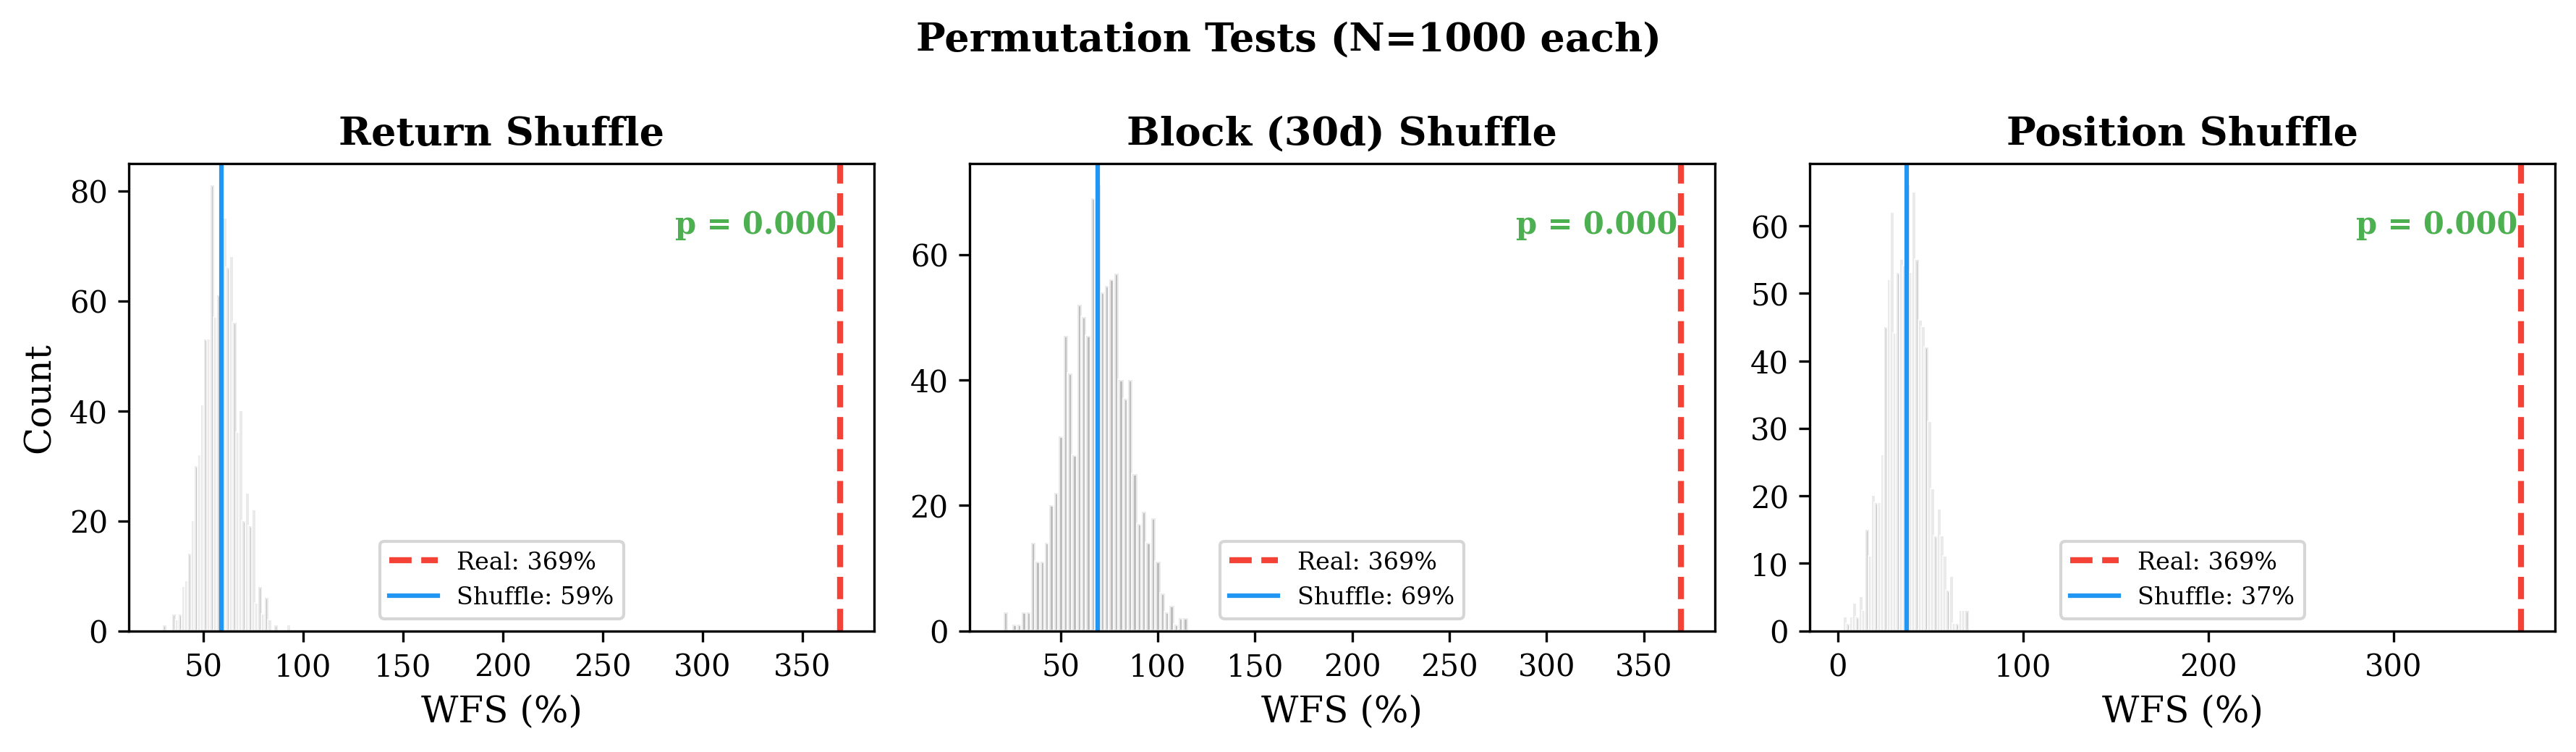
\includegraphics[width=\textwidth]{../figures/paper/fig7_shuffle_tests.png}
\caption{Permutation test distributions ($N=1{,}000$ each). Red dashed: real WFS (369\%). Blue solid: shuffle mean. All three tests yield $p=0.000$, though we note that shuffling destroys temporal structure, setting a low bar for significance.}
\label{fig:shuffle}
\end{figure}

\begin{figure}[htbp]
\centering
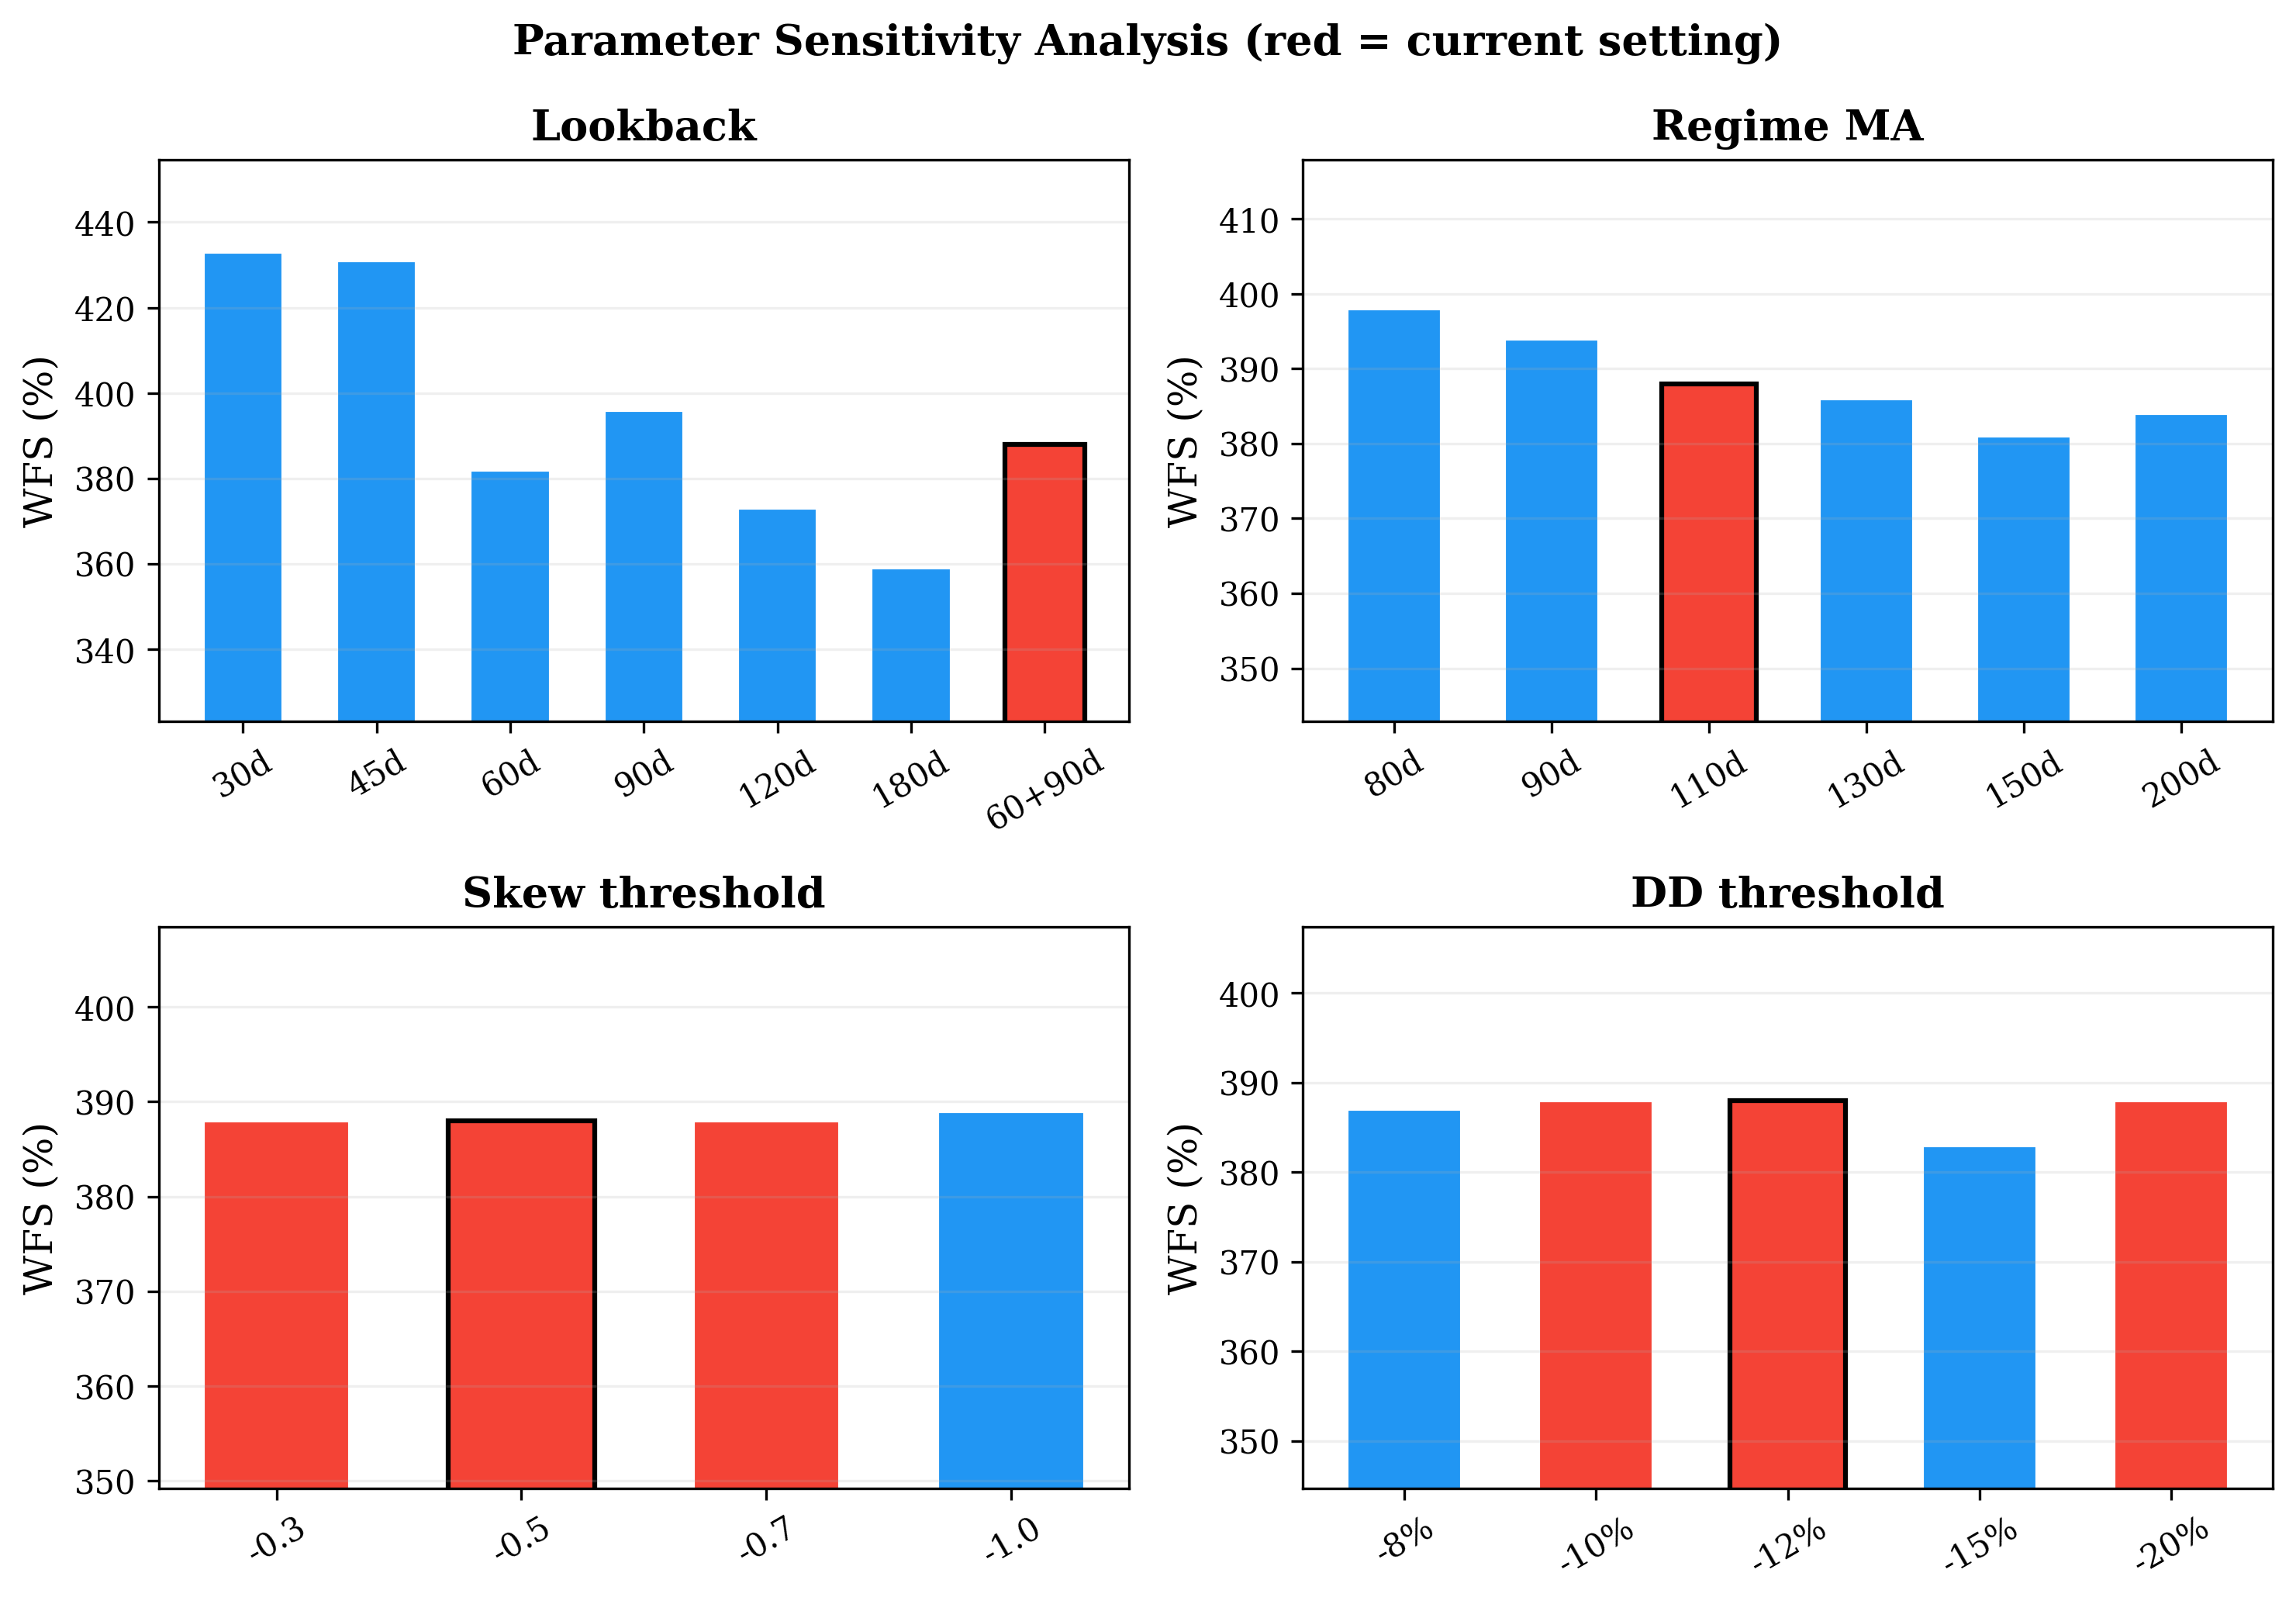
\includegraphics[width=0.9\textwidth]{../figures/paper/fig8_param_sensitivity.png}
\caption{Parameter sensitivity analysis. Red bars indicate current settings. WFS remains within $\pm 10\%$ of the baseline across all parameter perturbations, demonstrating robustness to individual parameter choices.}
\label{fig:sensitivity}
\end{figure}

Table~\ref{tab:stats} summarizes all statistical tests. The permutation tests confirm that position timing contains information ($p=0.000$), but we caution that shuffling destroys autocorrelation and volatility clustering, setting a low hurdle. The more stringent $t$-test for WFS $> 300\%$ yields $p=0.206$ and cannot be rejected at conventional significance levels. The statistically defensible claims are: (1) the win rate exceeds 50\% ($p<0.0001$), and (2) the strategy generates positive returns in a down market (OOS 2025: $+93\%$ vs.\ BTC $-7\%$).

Alpha decay analysis reveals a statistically significant declining trend ($p=0.003$), consistent with increasing market efficiency in cryptocurrency markets.

% ============================================================
\section{Discussion}
\label{sec:discussion}

\begin{figure}[htbp]
\centering
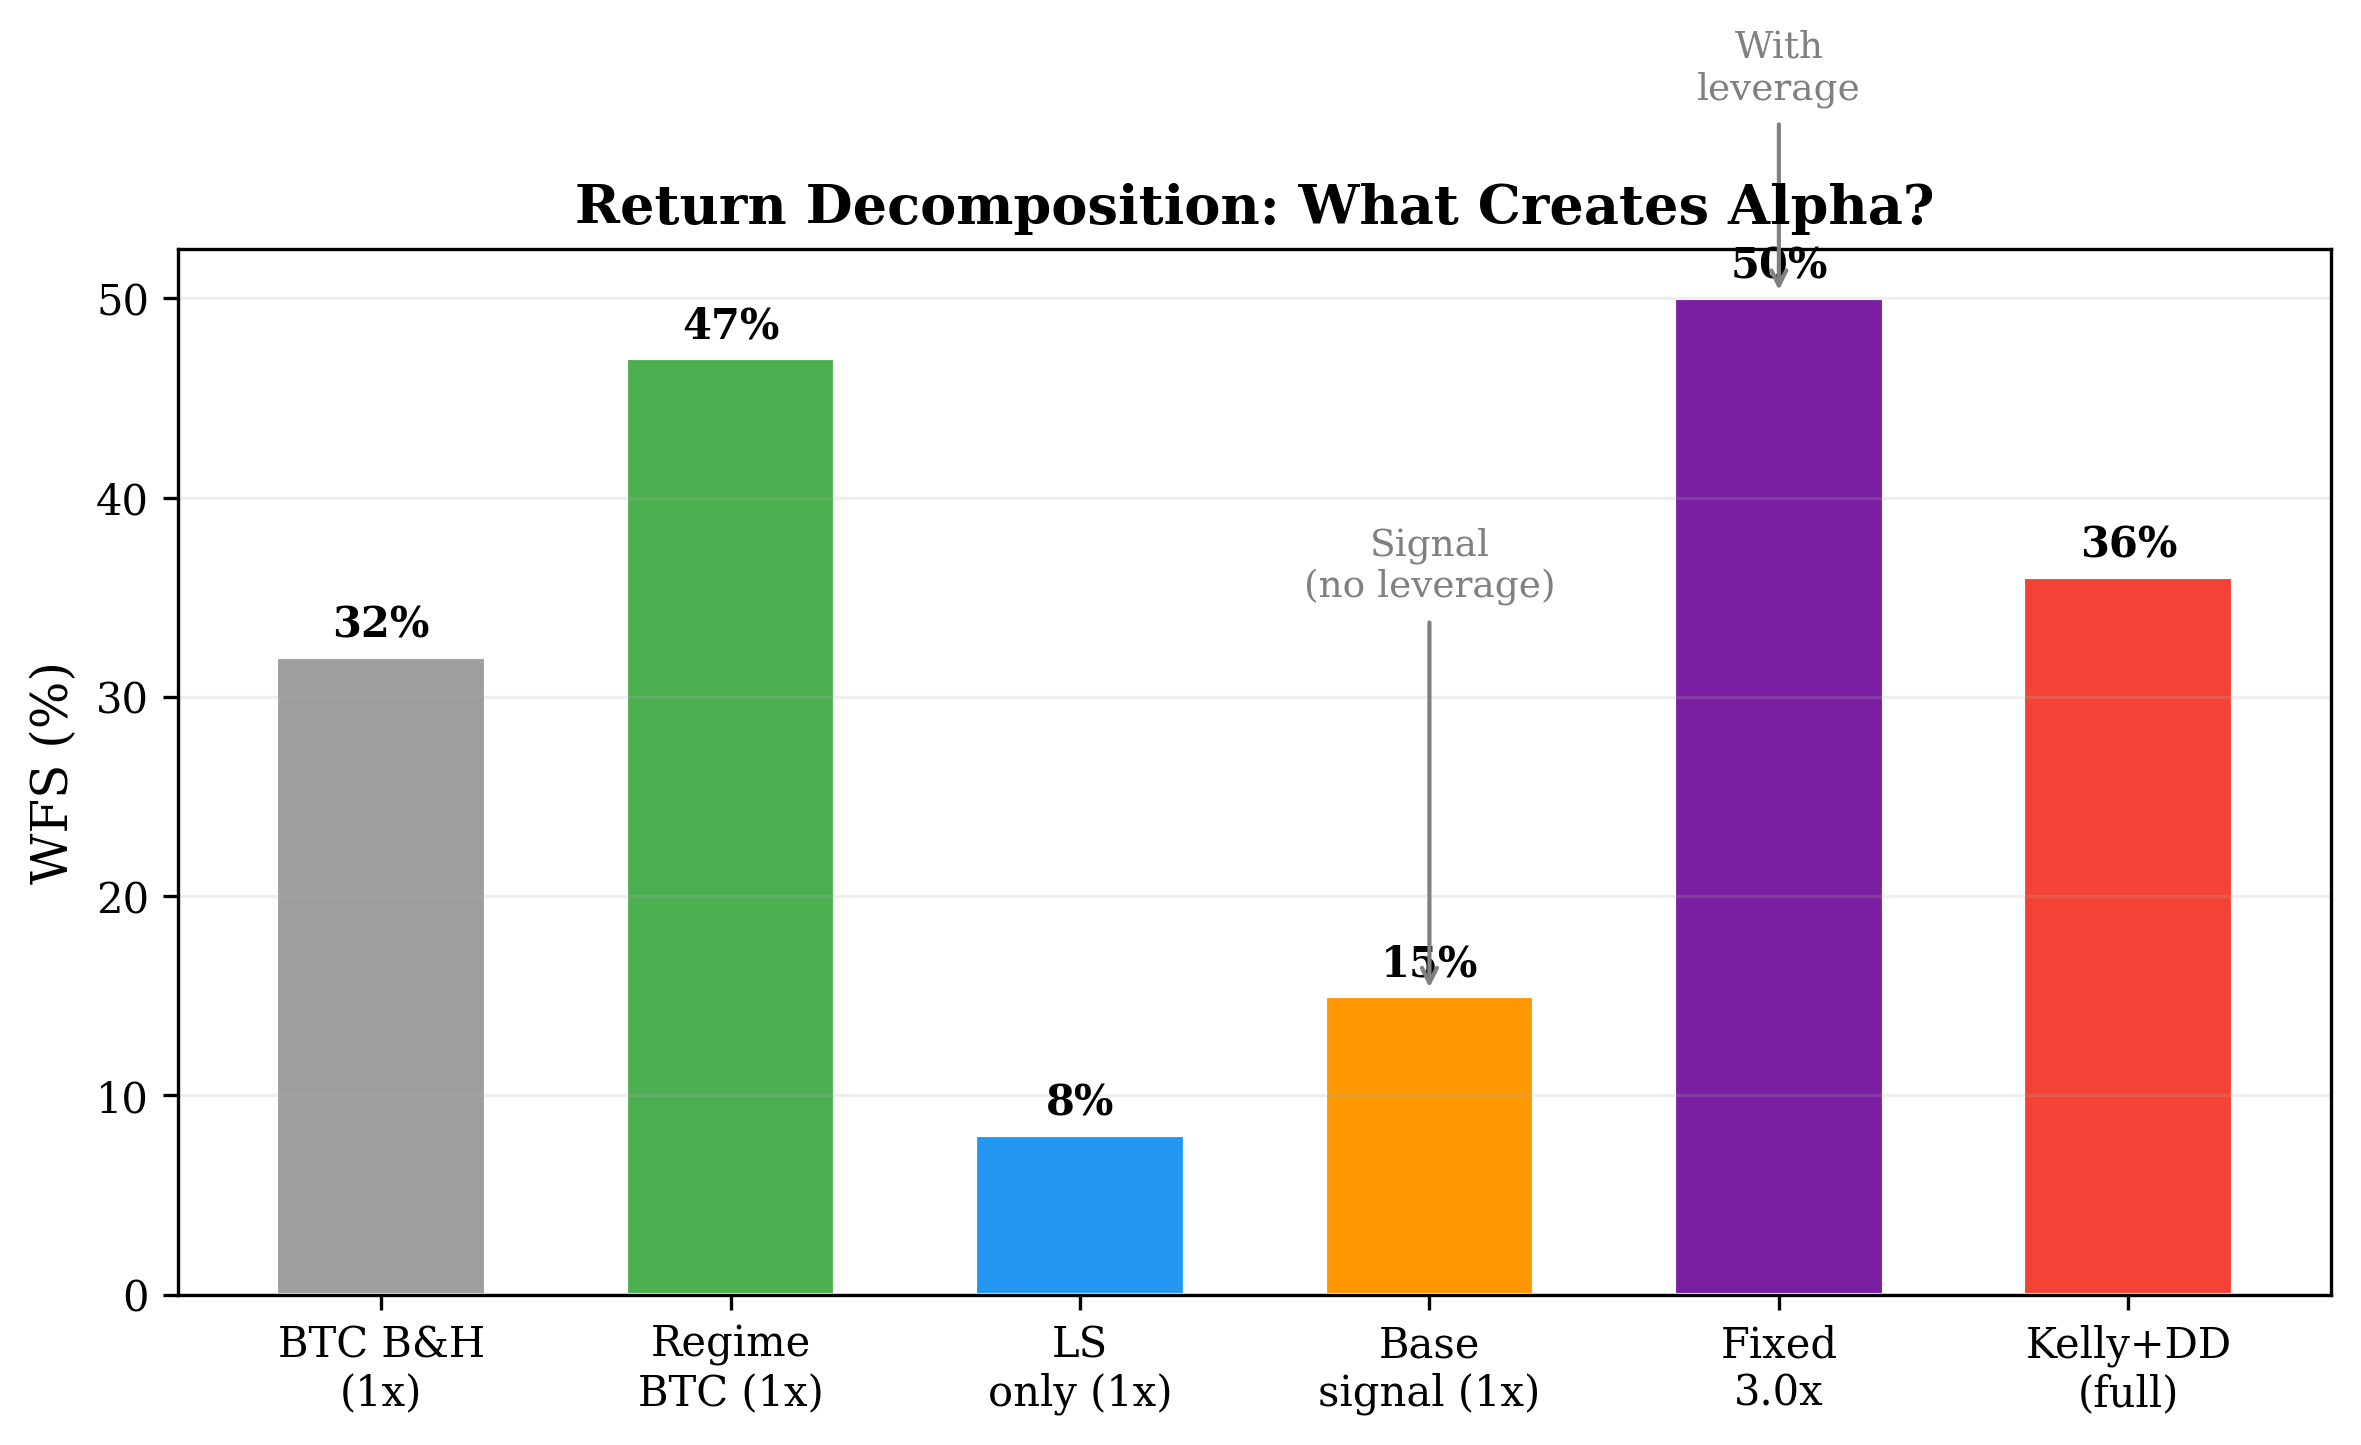
\includegraphics[width=0.85\textwidth]{../figures/paper/fig9_decomposition.png}
\caption{Return decomposition. At 1$\times$ leverage, the base signal (regime + LS blend) yields WFS $+15\%$, below BTC Buy \& Hold ($+32\%$). The model's value is not directional alpha but crash protection that enables safe leverage application.}
\label{fig:decomposition}
\end{figure}

\subsection{Source of Returns}
At $1\times$ leverage, the unblended signal underperforms buy-and-hold (Figure~\ref{fig:decomposition}). The model's value lies in making leverage \emph{survivable}: BTC at $3\times$ leverage would have been liquidated in 2022 ($-65\% \times 3 = -195\%$), while RACM at $3\times$ returned $+121\%$. The regime detection system acts as crash protection---analogous to a seatbelt that does not make a car faster but enables safe high-speed driving.

\subsection{The Leverage Illusion}
The IS WFS of 367\% is partially an artifact of $3\times$ leverage applied to hourly compounding over 4 years. The position cap of $3.0\times$ was selected from a sweep, introducing result-dependence. At cap $= 2.5\times$ (a less data-dependent choice), WFS is $290\%$. Removing the three most extreme folds reduces WFS from 367\% to 253\%.

\subsection{Practical Constraints}
The strategy's capacity is limited to approximately \$50K--\$200K due to DEX liquidity constraints. Execution uses Binance data for signal generation and Lighter.xyz for order execution, creating a cross-exchange basis risk of 2--5 bps normally, potentially 50--100 bps during high volatility.

\subsection{Structural Weakness}
The strategy fails when all assets move in perfect correlation (Luna crash, FTX collapse, JPY carry unwind). In these events, the LS spread collapses. However, losses are contained to $-4.0\%$ per fold maximum, and recovery occurs within 2--3 months.

% ============================================================
\section{Conclusion}
\label{sec:conclusion}

We present RACM, a regime-adaptive cross-sectional momentum strategy for cryptocurrency markets. The strategy's primary contribution is demonstrating that momentum-based risk management enables safe leverage in a highly volatile asset class. Our statistically defensible claims are:
\begin{enumerate}
\item A fold win rate of 87\% significantly exceeding 50\% ($p<0.0001$)
\item Positive out-of-sample returns ($+93\%$) in a BTC-declining year ($-7\%$)
\item Robustness to parameter perturbation (9 out of 9 tests pass)
\item A 21-point leak prevention protocol with all items verified
\end{enumerate}

What we \emph{cannot} claim statistically is WFS $> 300\%$ ($p=0.206$). Alpha shows a significant declining trend ($p=0.003$), suggesting that the strategy's edge may erode over 2--3 years as cryptocurrency markets mature. Future work includes weekly walk-forward validation for larger fold counts, adaptive cap selection, and live trading validation.

% ============================================================
\section*{Acknowledgments}
The author thanks [Advisor Name] for valuable guidance and feedback throughout this research.

\section*{Data Availability Statement}
Price data are publicly available from the Binance API (\url{https://api.binance.com}). Historical derivatives data (funding rates, open interest, liquidation counts) were obtained from Tardis (\url{https://tardis.dev}). The complete backtest code and analysis scripts are available at \url{https://github.com/nanashiNiA/regime-adaptive-crypto-momentum}.

\section*{Declaration of Interest}
The author declares no competing financial interests or personal relationships that could have influenced the work reported in this paper.

\noindent\textbf{JEL Classification:} G11 (Portfolio Choice), G14 (Information and Market Efficiency), C58 (Financial Econometrics)

% ============================================================
\bibliographystyle{plainnat}
\bibliography{references}

% ============================================================
\appendix
\section{45-Fold Walk-Forward Detailed Results}
\label{app:folds}

\begin{table}[htbp]
\centering
\caption{Complete 45-Fold Walk-Forward Results (cap = 3.0$\times$, KF = 0.15)}
\label{tab:all_folds}
\small
\begin{tabular}{rlrrl|rlrrl}
\toprule
\# & Period & Return & MaxDD & Res. & \# & Period & Return & MaxDD & Res. \\
\midrule
1  & 2021-04 & $+255.7$ & $-7.1$ & W & 24 & 2023-03 & $+25.5$ & $-5.4$ & W \\
2  & 2021-05 & $+98.5$  & $-15.7$ & W & 25 & 2023-04 & $+5.6$  & $-3.8$ & W \\
3  & 2021-06 & $+3.4$   & $-9.2$ & W & 26 & 2023-05 & $+9.8$  & $-3.1$ & W \\
4  & 2021-07 & $+5.6$   & $-11.3$ & W & 27 & 2023-06 & $+22.6$ & $-4.8$ & W \\
5  & 2021-08 & $+47.6$  & $-6.2$ & W & 28 & 2023-07 & $+3.5$  & $-9.4$ & W \\
6  & 2021-09 & $+44.5$  & $-7.1$ & W & 29 & 2023-08 & $+2.1$  & $-4.4$ & W \\
7  & 2021-10 & $+63.6$  & $-5.0$ & W & 30 & 2023-09 & $+5.8$  & $-3.3$ & W \\
8  & 2021-11 & $+66.1$  & $-4.6$ & W & 31 & 2023-10 & $+31.9$ & $-3.3$ & W \\
9  & 2021-12 & $-1.0$   & $-9.4$ & L & 32 & 2023-11 & $+25.4$ & $-6.0$ & W \\
10 & 2022-01 & $+10.9$  & $-10.0$ & W & 33 & 2023-12 & $+69.5$ & $-5.2$ & W \\
11 & 2022-02 & $+17.4$  & $-3.4$ & W & 34 & 2024-01 & $+27.5$ & $-5.6$ & W \\
12 & 2022-03 & $+4.0$   & $-10.1$ & W & 35 & 2024-02 & $+72.1$ & $-2.5$ & W \\
13 & 2022-04 & $-0.1$   & $-10.5$ & L & 36 & 2024-03 & $+134.5$ & $-4.3$ & W \\
14 & 2022-05 & $-3.6$   & $-12.1$ & L & 37 & 2024-04 & $+5.9$  & $-6.7$ & W \\
15 & 2022-06 & $+16.1$  & $-5.6$ & W & 38 & 2024-05 & $+7.4$  & $-5.1$ & W \\
16 & 2022-07 & $+26.0$  & $-4.1$ & W & 39 & 2024-06 & $+12.9$ & $-3.0$ & W \\
17 & 2022-08 & $-3.3$   & $-9.9$ & L & 40 & 2024-07 & $+26.4$ & $-3.5$ & W \\
18 & 2022-09 & $+10.7$  & $-6.1$ & W & 41 & 2024-08 & $-2.7$  & $-10.2$ & L \\
19 & 2022-10 & $+45.0$  & $-6.5$ & W & 42 & 2024-09 & $+3.6$  & $-4.6$ & W \\
20 & 2022-11 & $-4.0$   & $-14.1$ & L & 43 & 2024-10 & $+37.4$ & $-3.5$ & W \\
21 & 2022-12 & $+1.5$   & $-7.6$ & W & 44 & 2024-11 & $+56.6$ & $-7.9$ & W \\
22 & 2023-01 & $+52.4$  & $-4.8$ & W & 45 & 2024-12 & $+24.0$ & $-5.8$ & W \\
23 & 2023-02 & $+12.7$  & $-6.0$ & W &    &         &         &        &   \\
\bottomrule
\end{tabular}
\begin{tablenotes}
\small
\item Returns and MaxDD in percent. W = Win (positive return), L = Lose. Total: 39W / 6L.
\end{tablenotes}
\end{table}

\end{document}
